\documentclass{standalone}
\usepackage{tikz}
\usetikzlibrary{shapes,arrows, positioning,matrix,calc, fit, decorations.markings}

\pgfdeclarelayer{bg} % declare foreground layer
\pgfsetlayers{bg,main} % set layer order

\hyphenpenalty=10000
% https://texample.net/tikz/examples/simple-flow-chart/
% Define block styles
\tikzstyle{block} = [rectangle, draw, fill=blue!20, text centered, minimum height=1.25cm, outer sep=0pt, inner sep=0pt, anchor=center, text width=2.5cm]
\tikzstyle{innerblock} = [rectangle, draw, fill=red!20, outer sep=0pt, inner sep=0pt, minimum height=2.25cm, text width=10cm]
\tikzstyle{block2} = [rectangle, draw, fill=blue!20, text centered, minimum height=0.75cm, outer sep=0pt, inner sep=0pt, anchor=center, text width=2.5cm]
\tikzstyle{line} = [draw, -latex', line width=2pt]

\begin{document}
 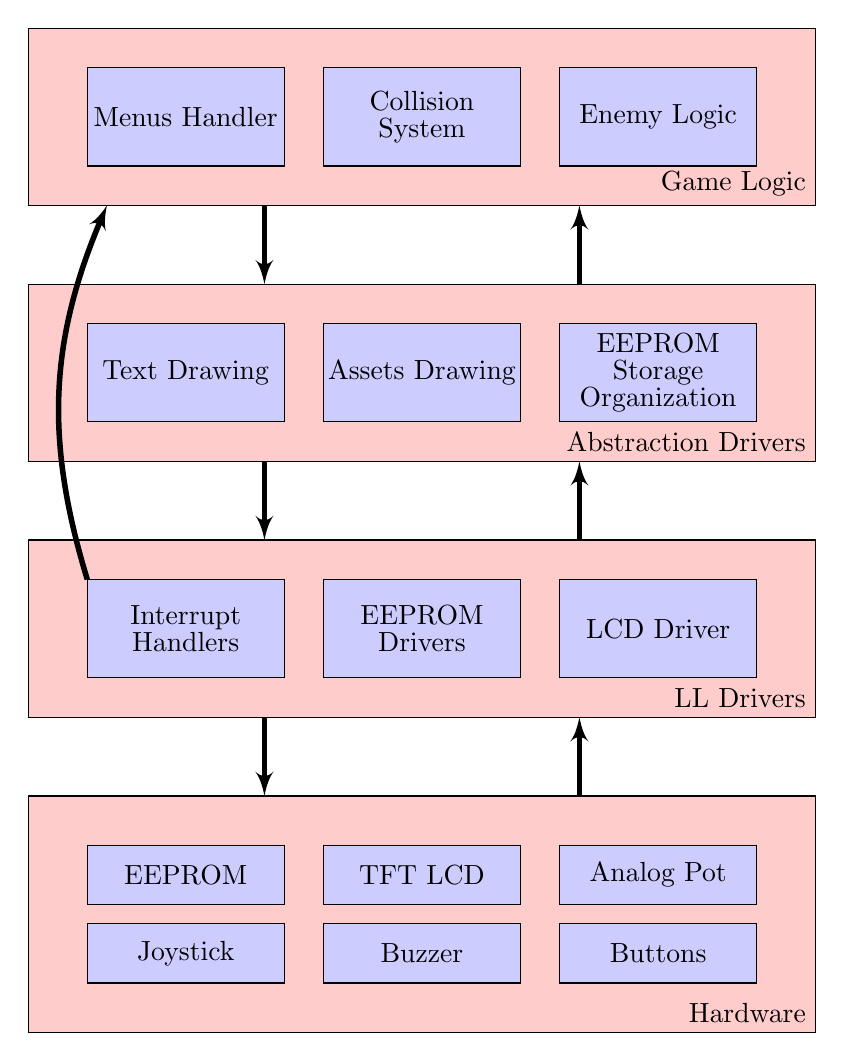
\begin{tikzpicture}[node distance=1cm]
    \renewcommand{\baselinestretch}{0.8}
    
    \node[innerblock] at (0,0) (ll) {};
    \node[anchor=south east] at (ll.south east) {LL Drivers};
    \node[block] at ($(ll.center)+(3,0)$) (lcddriver) {LCD Driver}; 
    \node[block] at ($(ll.center)+(0,0)$) {EEPROM Drivers};
    \node[block] at ($(ll.center)+(-3,0)$) (llinterrupt) {Interrupt Handlers};
    
    \node[innerblock, above=of ll] (mid) {};
    \node[anchor=south east] at (mid.south east) {Abstraction Drivers};
    \node[block] at ($(mid.center)+(0,0)$) {Assets Drawing};
    \node[block] at ($(mid.center)+(-3,0)$) {Text Drawing};
    \node[block] at ($(mid.center)+(3,0)$) {EEPROM Storage Organization};
    
    \node[innerblock, above=of mid] (game) {};
    \node[anchor=south east] at (game.south east) {Game Logic};
%     \node[block] at (-3,6) {Score System};
    \node[block] at ($(game.center)+(-3,0)$) {Menus Handler};
    \node[block] at ($(game.center)$) {Collision System};
    \node[block] at ($(game.center)+(3,0)$) {Enemy Logic};
    
    \node[innerblock, below=of ll, minimum height=3cm] (hard) {};
    \node[anchor=south east] at (hard.south east) {Hardware};
    \node[block2] at ($(hard.center)+(-3,-0.5)$) {Joystick};
    \node[block2] at ($(hard.center)+(3,-0.5)$) {Buttons};
    \node[block2] at ($(hard.center)+(-3,0.5)$) {EEPROM};
    \node[block2] at ($(hard.center)+(3,0.5)$) {Analog Pot};
    \node[block2] at ($(hard.center)+(0,0.5)$) {TFT LCD};
    \node[block2] at ($(hard.center)+(0,-0.5)$) {Buzzer};
    
    \begin{pgfonlayer}{bg}
        \draw[line] ([xshift=2cm]hard.north) to ([xshift=2cm]ll.south);
        \draw[line] ([xshift=-2cm]ll.south) to ([xshift=-2cm]hard.north);
        
        \draw[line] ([xshift=2cm]ll.north) to ([xshift=2cm]mid.south);
        \draw[line] ([xshift=-2cm]mid.south) to ([xshift=-2cm]ll.north);
        
        \draw[line] ([xshift=2cm]mid.north) to ([xshift=2cm]game.south);
        \draw[line] ([xshift=-2cm]game.south) to ([xshift=-2cm]mid.north);
    \end{pgfonlayer}
    
    \path[-latex', line width=2pt] (llinterrupt.north west) edge[bend left=20] ($(game.south west)+(1,0)$);
    
 \end{tikzpicture}
\end{document}
